\documentclass[12pt, a4paper, oneside]{ctexart}
\usepackage{amsmath, amsthm, amssymb, graphicx}
\usepackage{hyperref}
\usepackage{listings}
\usepackage{xcolor}
\usepackage{color}
\usepackage{enumerate}
\usepackage{epstopdf}
\usepackage{float}
\hypersetup{
    colorlinks=true,
    linkcolor=blue,
    filecolor=blue,      
    urlcolor=blue,
    citecolor=cyan,
}
\definecolor{dkgreen}{rgb}{0,0.6,0}
\definecolor{gray}{rgb}{0.5,0.5,0.5}
\definecolor{mauve}{rgb}{0.58,0,0.82}

\lstset{ %
    language=Python,                % the language of the code
    basicstyle=\footnotesize,           % the size of the fonts that are used for the code
    numbers=left,                   % where to put the line-numbers
    %numberstyle=\tiny\color{gray},  % the style that is used for the line-numbers
    %stepnumber=2,                   % the step between two line-numbers. If it's 1, each line 
                            % will be numbered
    %numbersep=5pt,                  % how far the line-numbers are from the code
    %backgroundcolor=\color{blue},      % choose the background color. You must add \usepackage{color}
    showspaces=false,               % show spaces adding particular underscores
    %showstringspaces=false,         % underline spaces within strings
    showtabs=false,                 % show tabs within strings adding particular underscores
    frame=single,                   % adds a frame around the code
    rulecolor=\color{black},        % if not set, the frame-color may be changed on line-breaks within not-black text (e.g. commens (green here))
    tabsize=2,                      % sets default tabsize to 2 spaces
    captionpos=b,                   % sets the caption-position to bottom
    breaklines=true,                % sets automatic line breaking
    breakatwhitespace=false,        % sets if automatic breaks should only happen at whitespace
    title=\lstname,                   % show the filename of files included with \lstinputlisting;
                            % also try caption instead of title
    keywordstyle=\color{blue},          % keyword style
    commentstyle=\color{dkgreen},       % comment style
    stringstyle=\color{mauve},         % string literal style
    escapeinside={\%*}{*)},            % if you want to add LaTeX within your code
    morekeywords={*,...}               % if you want to add more keywords to the set
}
\title{Machine Learning Lab2}
\author{Xiaoma}
\date{2022.10.18}
\begin{document}
\maketitle
\section*{实验要求}
\begin{enumerate}
    \item 独立编写SVM解决二分类问题
    \item 采用两种不同方法解决二次规划问题(禁止使用sklearn或其他机器学习库)
    \item 测试代码效率并与标准库进行比较
\end{enumerate}
\href{https://github.com/gsb-ustc/CS231n-2020-assignment-solution}{参考曾在课外完成的cs231n-assignment1}

\section*{实验原理}
\subsection*{SVM}
线性SVM
\begin{itemize}
    \item 硬边距:\\
    给定数据和标签:$X,y$,硬边界SVM是在线性可分问题中求解最大边距超平面的算法,约束条件是样本点到决策
    边界的距离大于等于1.硬边距SVM可以转化为一个等价的二次凸优化问题进行求解
    $$\min_{w,b} \frac{1}{2}\| w\Vert^{2} $$
    $$s.t. \quad y_{i}(w^{T}X_{i}+b) \geq 1$$
    \item 软边距:\\
    在线性不可分问题中使用硬边距SVM将产生分类误差,因此可在最大化边距的基础上引入损失函数构造新的优化问题,
    当使用松弛变量处理损失函数时,软边距SVM的优化问题为
    $$\min_{w,b} \frac{1}{2}\| w\Vert^{2}+C\sum_{i=1}^{N}\xi _{i}$$
    $$s.t. \quad y_{i}(w^{T}X_{i}+b) \geq 1 - L_{i},L_{i}\geq 0 $$
\end{itemize}
\subsection*{SMO}
SMO是一种坐标下降法,以迭代方式求解SVM的对偶问题,其设计是在每个迭代步选择拉格朗日
乘子中的两个变量$\alpha_{i},\alpha_{j}$ 并固定其它参数,将原优化问题化简至1维子可行域,此时约束条件有如下等价形式
$$\sum_{i=1}^{N}\alpha_{i}y_{i}=0 \Longleftrightarrow \alpha_{i}y_{i}+\alpha_{j}y_{j}=-\sum_{k\neq i,j}\alpha_{k}y_{k}=const$$
SMO的计算框架:
\begin{enumerate}
    \item 初始所有化拉格朗日乘子
    \item 识别一个不满足KKT条件的乘子,并求解其二次规划问题
    \item 反复执行上述步骤直到所有乘子满足KKT条件或参数的更新量小于设定值
\end{enumerate}
\subsection*{SGD}
从损失函数优化的角度来解决这个问题,我们构建一种hinge损失函数
$$L(w,b)=\sum_{i}\max(0,1-y_{i}(wx_{i}+b))$$
正确分类并且置信度$y_{i}(wx_{i}+b)$大于1的样本点对损失函数的贡献为0,而其他样本点会
对损失函数产生影响,从而在优化损失函数的时候有针对地调整。对于这样在开放空间上的参数解,
我们通常都会增加一个正则项,以降低最终参数的复杂度。那么最终使用的损失函数
$$L(w,b)=\sum_{i}\max(0,1-y_{i}(wx_{i}+b))+\frac{1}{C}\|w\Vert^{2}$$
\section*{实现细节}
\subsection*{(SVM1)SVM-SGD}
\subsubsection*{class SVM1}
\begin{itemize}
    \item self.w : 权重矩阵
    \item self.loss : hinge损失
    \item self.dw : 权重梯度
\end{itemize}
\begin{lstlisting}
    def __init__(self):
        self.w = None
        self.loss = None
        self.dw = None
\end{lstlisting}

\subsubsection*{svm\_loss}
计算hinge损失与梯度
\begin{lstlisting}
    def svm_loss(self, w, x, y, reg):
        loss = 0.0
        
        dw = np.zeros(w.shape)
        num_train = x.shape[0]
        scores = x.dot(w)
        #print(scores[range(num_train), y[0]])
        correct_class_scores = scores[ np.arange(num_train), list(y)].reshape(num_train,1)
        margin = np.maximum(0, scores - correct_class_scores +1)
        margin[range(num_train), list(y)] = 0
        data_loss = np.sum(margin)*1.0 / num_train
        reg_loss = reg * np.sum(np.square(w))
        loss = data_loss + reg_loss
        
        x_effect = (margin > 0).astype('float')
        x_effect[range(num_train), y] -= np.sum(x_effect, axis=1)
        dw = x.T.dot(x_effect)
        dw /= num_train
        dw += 2*reg*w
        
        return loss, dw
\end{lstlisting}

\subsubsection*{fit}
使用SGD算法训练模型,考虑到数据集参数过大,可采用每次训练抽取其中一部分数据进行梯度下降的方式。
\begin{itemize}
    \item x : 训练数据参数
    \item y : 训练数据标签
    \item batch\_size : 随机抽取的数据数量
    \item reg : 正则化参数
    \item learning\_rate : 学习率
    \item num\_iters : 最大训练次数
\end{itemize}
\begin{lstlisting}
    def fit(self, x, y, learning_rate, reg, num_iters, batch_size, verbose):
        """
        Fit the coefficients via your methods
        """ 
        y = y.astype('int')
        y[:] = (y[:] - np.min(y[:])) / (np.max(y[:]) - np.min(y[:]))
        for i in range(5):
            print(y[i])
        num_classes = 2
        num_train = x.shape[0]
        if self.w is None:
            self.w = 0.001 * np.random.randn(x.shape[1], num_classes)
            
        loss_history = []
        for it in range(num_iters):
            x_batch = None
            y_batch = None
            batch_idx = np.random.choice(num_train, size=batch_size, replace=False)
            x_batch = x[batch_idx]
            y_batch = y[batch_idx]
            #w_batch = self.w[batch_idx]
            #self.w = self.w
            #self.w = np.array(self.w).reshape(num_train, num_classes)
            loss, dw = self.svm_loss(self.w, x_batch, y_batch, reg)

            loss_history.append(loss)
            self.w -= learning_rate * dw
            if verbose and it % 100 == 0:
                print('iteration %d / %d  loss :' % (it, num_iters))
                print(loss)
            if loss < 0.2:
                break
        return loss_history    
\end{lstlisting}

\subsubsection*{predict}
使用训练得到的模型进行预测
\begin{itemize}
    \item x : 待预测数据
\end{itemize}
\begin{lstlisting}
    def predict(self, X):
        """
        Use the trained model to generate prediction probabilities on a neself.w
        collection of data points.
        """
        y_pred = np.zeros(X.shape)
        y_pred = np.argmax(X.dot(self.w), axis=1)
        return y_pred
\end{lstlisting}
\subsection*{(SVM2)SVM-SMO}
\subsubsection*{class SVM2}
\begin{itemize}
    \item self.w : 权重矩阵
    \item self.c : 正则化参数
    \item self.alpha : 拉格朗日乘子
    \item self.b : 常数b
    \item self.loss : 损失
\end{itemize}
\begin{lstlisting}
    def __init__(self):
        self.w = None
        self.c = None
        self.alpha = None
        self.b = 0
        self.loss = []
\end{lstlisting}

\subsubsection*{clip}
对$\alpha$进行剪枝,使其值在H,L之间
\begin{lstlisting}
    def clip(self, alpha, L, H):
        
        if alpha < L:
            return L
        elif alpha > H:
            return H
        else:
            return alpha
\end{lstlisting}

\subsubsection*{select\_j}
采用随机选择的方式选择参数$\alpha_{j}$
\begin{lstlisting}
    def select_j(self, i, m):
        l = list(range(m))
        seq = l[: i] + l[i+1:]
        return random.choice(seq)
\end{lstlisting}
\subsubsection*{f}
根据线性核函数计算预测值
\begin{lstlisting}
    def f(self, x_i, x, y):
        x_i = np.array(x_i).T
        data = np.array(x)
        ks = np.dot(data, x_i)
        wx = np.dot((self.alpha*y), ks)
        fx = wx + self.b
        return fx
\end{lstlisting}

\subsubsection*{fit}
使用SMO算法训练模型,由于随机选择$\alpha_{j}$的缘故,训练速度很慢
\begin{itemize}
    \item x : 训练数据参数
    \item y : 训练数据标签
    \item C : 软间隔常数
    \item max\_iter : 最大训练次数
\end{itemize}
\begin{lstlisting}
    def fit(self, x, y, C, max_iter):
        x = np.array(x)
        m, n = x.shape
        y = np.array(y)
        self.alpha = np.zeros(m)
        self.b = 0
        self.c = C
        it = 0

        while it < max_iter:
            pair_changed = 0
            for i in range(m):
                a_i, x_i, y_i = self.alpha[i], x[i], y[i]
                fx_i = self.f(x_i, x, y)
                loss_i = fx_i - y_i
                j = self.select_j(i, m)
                a_j, x_j, y_j = self.alpha[j], x[j], y[j]
                fx_j = self.f(x_j, x, y)
                loss_j = fx_j - y_j
                K_ii, K_jj, K_ij = np.dot(x_i, x_i), np.dot(x_j, x_j), np.dot(x_i, x_j)
                eta = K_ii + K_jj - 2*K_ij
                if eta <= 0:
                    continue
                a_i_old, a_j_old = a_i, a_j
                a_j_new = a_j_old + y_j*(loss_i - loss_j)/eta
                if y_i != y_j:
                    L = max(0, a_j_old - a_i_old)
                    H = min(self.c, self.c + a_j_old - a_i_old)
                else:
                    L = max(0, a_i_old + a_j_old - self.c)
                    H = min(self.c, a_j_old + a_i_old)
                a_j_new = self.clip(a_j_new, L, H)
                a_i_new = a_i_old + y_i*y_j*(a_j_old - a_j_new)
                if abs(a_j_new - a_j_old) < 0.00001:
                    continue
                self.alpha[i], self.alpha[j] = a_i_new, a_j_new
                b_i = -loss_i - y_i*K_ii*(a_i_new - a_i_old) - y_j*K_ij*(a_j_new - a_j_old) + self.b
                b_j = -loss_j - y_i*K_ij*(a_i_new - a_i_old) - y_j*K_jj*(a_j_new - a_j_old) + self.b
                if 0 < a_i_new < self.c:
                    self.b = b_i
                elif 0 < a_j_new < self.c:
                    self.b = b_j
                else:
                    self.b = (b_i + b_j)/2
                pair_changed += 1
                loss = 0
                #for i in range(m):
                #    loss += abs(self.f(x[i], x, y) - y[i])
                #self.loss.append(loss / m)
                
            if pair_changed <= 5:
                it += 1
            else:
                it = 0
            print('iteration:{}  pair_changed:{}'.format(it, pair_changed))
            self.get_w(x, y)
        return self.loss


\end{lstlisting}

\subsubsection*{predict}
使用训练得到的模型进行预测
\begin{itemize}
    \item x : 待预测数据
\end{itemize}

\begin{lstlisting}
    def predict(self, x):
        y_pred = np.zeros(x.shape)
        y_pred = x.dot(self.w) + self.b
        m = y_pred.shape[0]
        for i in range(m):
            if y_pred[i] >= 0:
                y_pred[i] = 1.0
            else:
                y_pred[i] = -1.0
        return y_pred
\end{lstlisting}
\section*{性能分析}

\subsection*{SVM-SGD}
\textbf{参数信息}\\
\textbf{样本数量:10000,维度:20,错标率:0.0375}\\
\textbf{learning\_rate : 1e-9\\reg : 2.5e4\\ num\_iters : 150000\\ batch\_size : 500}\\

\subsubsection*{loss曲线}
\begin{figure}[H]
    \centering
    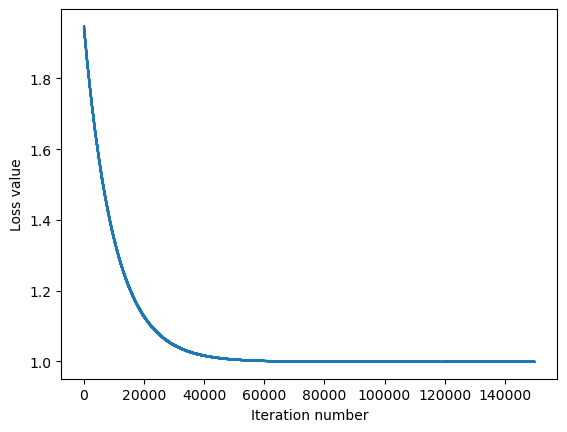
\includegraphics[scale=0.8]{sgd.png}
\end{figure}
\textbf{训练时间 :90.56s}\\
\textbf{训练精确度:0.945375}\\
\textbf{预测精确度:0.946000}

\subsection*{SVM-SMO}
\textbf{参数信息}\\
\textbf{样本数量:500,维度:20,错标率:0.0375}\\
\textbf{C : 0.7\\max\_iter : 40}\\
\textbf{训练时间 :667.76s}\\
\textbf{训练精确度:0.955000}\\
\textbf{预测精确度:0.930000}\\

\textbf{参数信息}\\
\textbf{样本数量:10000,维度:20,错标率:0.0375}\\
\textbf{C : 0.7\\max\_iter : 40}\\
\textbf{训练时间(使用了云服务器) :12.5h}\\
\textbf{训练精确度:0.95374}\\
\textbf{预测精确度:0.94230}

\subsubsection*{sklearn-SVM}
\textbf{参数信息}\\
\textbf{样本数量:10000,维度:20,错标率:0.0375}\\
\textbf{C : 0.7\\max\_iter : 40}\\
\textbf{训练时间 :1.20s}\\
\textbf{训练精确度:0.96725}\\
\textbf{预测精确度:0.943}
\section*{实验反思}
采用随机选择$\alpha_{j}$的方法代码过于繁琐,此外由于随机选择的原因,导致计算量过大,训练时间过长。
事实上SMO算法应采用优化的内循环方法,结合$\alpha_{j}$上次是否被替换过以及$\alpha_{j}$是否为0考虑,
由于个人能力原因未能完成内循环的SMO算法的实现。

\end{document}